\documentclass[11pt,a4paper]{article}
 
\usepackage[T1]{fontenc}
\usepackage[portuguese]{babel}
\usepackage{authblk}
\usepackage{enumitem}
\usepackage{graphicx}
\usepackage[hmargin=2cm,vmargin=3.5cm,bmargin=2cm]{geometry}
\usepackage[utf8]{inputenc}

\newcommand{\select}{\mbox{\Large$\sigma$}}

\pagenumbering{arabic}

\title{\textbf{Projecto de Bases de Dados, Parte 1}}
 
\author{Bruno Cardoso, Lídia Freitas e Rodrigo Bernardo} 

\affil{Instituto Superior T\'{e}cnico}

\begin{document}

\date{25 horas de trabalho por aluno.}

\maketitle

\centerline{
\includegraphics[width=0.4\textwidth]{ist-simbolo.jpg}}
\newpage

\tableofcontents
\newpage

\section{Modelo Entidade-Associa\c{c}\~ao}
\subsection{O Modelo}

\centerline{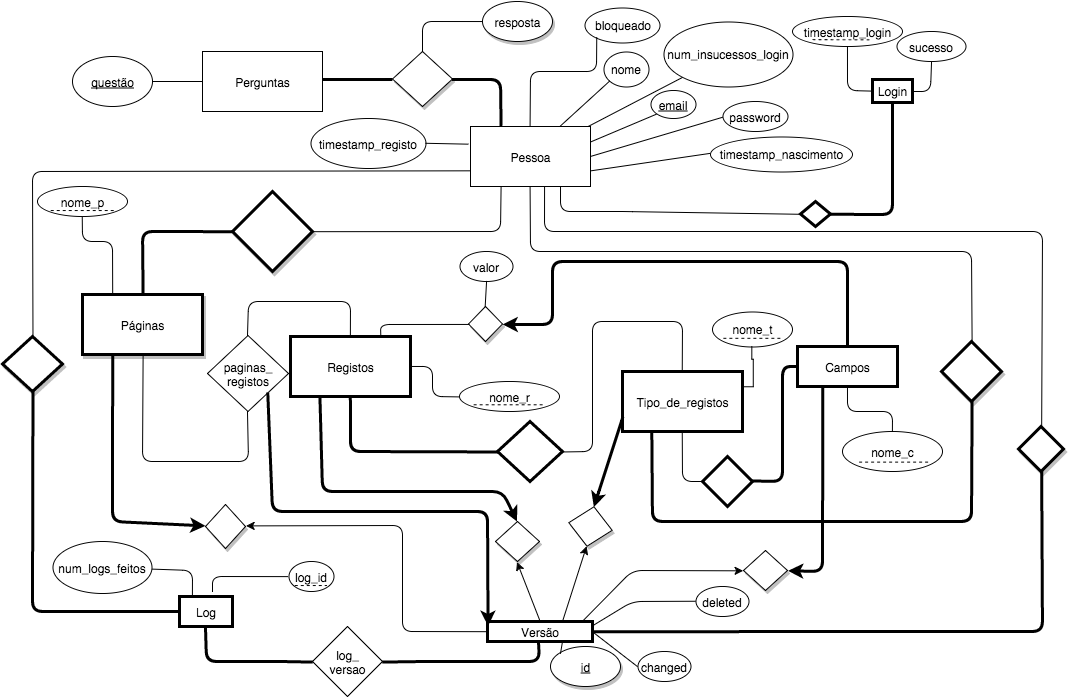
\includegraphics[width=1.0\textwidth]{modelo-ea.png}}

\newpage

\subsection{Restri\c{c}\~oes de Integridade do Modelo Entidade-Associa\c{c}\~ao}

\paragraph{}

O Modelo Entidade-Associação não limita todas as ocorrências possíveis e por isso podem dar-se situações fora do domínio do problema.

\\Como por exemplo, não se consegue assegurar que a ordem das datas estejam coerentes. Isto é, não é possível garantir que o timestamp\_nascimento seja inferior ao timestamp\_registo, ou que o timestamp\_login seja posterior ao timestamp\_registo.
Assim como não é possível assegurar que os números de tentativas de insucesso (num\_insucessos\_login) sejam positivos, ou o número de undo’s já realizados pela pessoa (num\_undos).
Outro aspecto que não é explicável através do modelo é o número de perguntas a que a pessoa responde, ou a unicidade da associação entre os objectos mutáveis (Páginas, páginas\_registos, Registos, Tipos\_de\_registos e Campos).
De forma a impedir que tais situações não ocorram, o Modelo Entidade-Associação é completado com as seguintes restrições de integridade:
\\

\begin{description}
  \item[RI1] Na entidade Pessoa, o atributo timestamp\_nascimento \'{e} uma data anterior ao atributo timestamp\_registo.
  \item[RI2] Na entidade Pessoa, o atributo bloqueado \'{e} um valor l\'{o}gico, verdadeiro ou falso.


  \item[RI3] Na entidade Pessoa, o atributo num\_undos \'{e} um n\'{u}mero inteiro positivo.


  \item[RI4] Na entidade Pessoa, o atributo num\_insucessos\_login '{e} um n\'{u}mero inteiro positivo menor ou igual a 3.
  \item[RI5] Cada instância de Pessoa associa-se, em cada instante, a duas instâncias da entidade Pergunta.
  \item[RI6] Na entidade Login, o atributo timestamp\_login \'{e} uma data posterior ao atributo timestamp\_registo de Pessoa.
  \item[RI7] Na entidade Login, o atributo sucesso \'{e} um valor l\'{o}gico, verdadeiro ou falso.
  \item[RI8] Cada instância da entidade Versão tem apenas uma associação activa a P\'{a}ginas, paginas\_registos, Registos, Tipos\_de\_registos e Campos.
  \item[RI9] Na entidade Versão, o atributo deleted \'{e} um valor l\'{o}gico, verdadeiro ou falso.
  \item[RI10] Na entidade Versão, o atributo changed \'{e} um valor l\'{o}gico, verdadeiro ou falso.
  \item[RI11] Uma instância da entidade Versão est\'{a} associada a uma ou duas instâncias da entidade Log.
  \item[RI12] Uma instância da entidade Log está associada a duas e s\'{o} duas instâncias da entidade Versão.
  \item[RI13] Na entidade Log, o atributo log\_id \'{e} um inteiro positivo.
\end{description}

\newpage
\section{Modelo Relacional}
\subsection{O Modelo}

\begin{description}[noitemsep]
	\item Pergunta(\underline{quest\~ao, email}, resposta)
	\item email: FK(Pessoa)
	\item notnull(resposta)
\end{description}

\begin{description}[noitemsep]
	\item Pessoa(\underline{email}, bloqueado, nome, num\_insucessos\_login, password, timestamp\_nascimento, timestamp\_registo, num\_undos)
	\item notnull(email)
	\item notnull(bloqueado)
	\item notnull(nome)
	\item notnull(num\_insucessos\_login)
	\item notnull(password)
	\item notnull(timestamp\_nascimento)
	\item notnull(timestamp\_registo)
	\item notnull(num\_undos)
\end{description}

\begin{description}[noitemsep]
	\item Login(\underline{timestamp\_login, email}, sucesso)
	\item email: FK(Pessoa)
	\item notnull(sucesso)
\end{description}

\begin{description}[noitemsep]
	\item P\'{a}ginas(\underline{nome\_p, email}, id)
	\item email: FK(Pessoa)
	\item id: FK(Pessoa)
	\item notnull(id)
\end{description}

\begin{description}[noitemsep]
	\item P\'{a}ginas\_registos(\underline{nome\_p, email, nome\_r, nome\_t},id )
	\item nome\_p, email: FK(P\'{a}ginas)
	\item nome\_r, nome\_t, email: FK(Registos)
	\item id: FK(Vers\~{a}o)
	\item notnull(id)
\end{description}

\begin{description}[noitemsep]
	\item Registos(\underline{nome\_r, nome\_t, email}, id)
	\item nome\_t, email: FK(tipos\_de\_registos)
	\item id: FK(Vers\~{a}o)
	\item notnull(id)
\end{description}

\begin{description}[noitemsep]
	\item Tipo\_de\_registos(\underline{nome\_t, email}, id)
	\item email: FK(Pessoa)
	\item notnull(id)
	\item id: FK(Vers\~{a}o)
\end{description}
\newpage

\begin{description}[noitemsep]
	\item Campos(\underline{nome\_c, nome\_t, email}, id)
	\item nome\_t, email: FK(Tipo\_de\_registos)
	\item id: FK(Vers\~{a}o)
	\item notnull(id)
\end{description}

\begin{description}[noitemsep]
	\item Registo\_Campos(\underline{nome\_r, nome\_t, nome\_c, email}, id)
	\item nome\_r, nome\_t, email: FK(Registos)
	\item nome\_c, nome\_t, email: FK(Campos)
	\item id: FK(Vers\~{a}o)
	\item notnull(id)
\end{description}


\begin{description}[noitemsep]
	\item Vers\~{a}o(\underline{id}, changed, deleted)
	\item notnull(changed)
	\item notnull(deleted)
\end{description}

\begin{description}[noitemsep]
	\item Log(\underline{log\_id, email})
	\item email: FK(Pessoa)
\end{description}

\begin{description}[noitemsep]
	\item Log\_vers\~{a}o(\underline{log\_id, email, id})
	\item log\_id, email: FK(Log)
	\item id: FK(Vers\~{a}o)
\end{description}

\newpage

\subsection{Restri\c{c}\~oes de Integridade do Modelo Relacional}



\newpage
\section{\'{A}lgebra Relacional}
\subsection{Pergunta 1}

$\Pi_{nome\_t}(\sigma_{email = 'Manel@Notebook.pt'}(Tipo\_de\_registos))$

\subsection{Pergunta 2}

$\Pi_{email}$ (Pessoa $ \bowtie \select_{sucesso=falso} (Login)$ )

\subsection{Pergunta 3}

$\Pi_{timestamp\_nascimento}(\sigma_{nome\_p = 'facebook' \wedge nome\_r = 'facebook'} Pessoa \bowtie 
\\\rho( P, P\'{a}ginas) \bowtie_{P.email = R.email} \rho( R, Registos)) $

\section{Linguagem SQL}
\subsection{Pergunta 1}
SELECT DISTINCT nome\_t
\\FROM Tipo\_de\_registos
\\WHERE email="Manel@notebook.pt";

\subsection{Pergunta 2}
SELECT DISTINCT Pessoa.email 
\\FROM Pessoa, Login 
\\WHERE Pessoa.email = Login.email AND sucesso = false;

\subsection{Pergunta 3}
SELECT timestamp\_nascimento
\\FROM Pessoa, Paginas, Registos 
\\WHERE Pessoa.email = Registos.email 
\\AND Pessoa.email = Paginas.email 
\\AND nome\_p = "facebook" 
\\AND nome\_r = "facebook";








\end{document}